\documentclass[runningheads]{llncs}

\usepackage{booktabs}
\usepackage{xspace}
\usepackage{hyperref}
\usepackage{graphicx}
\usepackage{comment}
\usepackage{float}
\usepackage{lipsum}
\usepackage{amsmath}
\usepackage{soul}
\usepackage{xcolor}
\usepackage{mathtools}

\newcommand{\todo}[1]{\textcolor{red}{\textbf{TODO: #1}}}
\newcommand{\red}[1]{\textcolor{red}{#1}}
\newcommand{\blue}[1]{\textcolor{blue}{#1}}
\newcommand{\hide}[1]{}

\makeatletter
\renewcommand{\fps@figure}{!ht}
\renewcommand{\fps@table}{!ht}
\makeatother

\newenvironment{colorpar}[1]{%
    \leavevmode\color{#1}\ignorespaces%
}{%
}%


%% Some important configurations here %%
\graphicspath{{../images/}, {../plots/experiment_}, {../plots/}}

\DeclarePairedDelimiter\ceil{\lceil}{\rceil}
\DeclarePairedDelimiter\floor{\lfloor}{\rfloor}

\newcommand{\poa}{proof-of-authority\xspace}
\newcommand{\Poa}{Proof-of-authority\xspace}
\newcommand{\pow}{proof-of-work\xspace}
\newcommand{\Pow}{Proof-of-work\xspace}
\newcommand{\rpi}{Raspberry Pi Zero~W\xspace}
\newcommand{\rab}{range-and-bearing\xspace}


%% Title and authors %%
\title{Blockchain-based coordination of a foraging robot swarm} \titlerunning{Blockchain-based coordination of a foraging robot swarm}
\author{Alexandre Pacheco\orcidID{0000-0001-5933-3553} \and Volker
  Strobel\orcidID{0000-0003-2974-9827} \and Andreagiovanni Reina\orcidID{0000-0003-4745-992X} \and Marco
  Dorigo\orcidID{0000-0002-3971-0507}} \authorrunning{A. Pacheco et
  al.}  
  \institute{IRIDIA, Universit\'e Libre de Bruxelles, Brussels, Belgium
  \email{alexandre.melo.pacheco@ulb.ac.be}}

	\index{Pacheco, Alexandre}
	\index{Strobel, Volker}
	\index{Reina, Andreagiovanni}
	\index{Dorigo, Marco}

\date{\today}

\begin{document}
\maketitle

% Some quotes and outtakes
%Cooperative foraging is most beneficial when food resources are unpredictable or scarce, as cooperative groups are likely to locate and exploit resources with greater efficiency than individuals (Wilson 2000).


\section{Introduction}
\label{sec:introduction}
%In groups of larger animals, it often results from the prospect of mutual benefits -- or a competitive advantage -- when foraging as a group is more energy-efficient than foraging individually
Cooperative foraging is a group behavior that emerges when individuals work together to gather food resources more efficiently. One way to cooperate is to exchange information about resource locations, as observed in some insect colonies (such as fire ants, that deposit pheromones on trails leading to resource locations; and honey-bees that perform recruitment dances to signal other about resource locations). Recent studies show that foraging robot swarms can also benefit from cooperation. For example, the authors in \cite{pitonakova_understanding_2014,pitonakova_icr_2018} show that when resources are scarce or difficult to find, nest-site recruitment can be helpful to maximize the total resources collected. Conversely, in resource-abundant environments it may be more advantageous to forage individually, and thus prevent physical interference (when robots foraging for the same resources collide) and informational interference (when the information exchanged is outdated, or incorrect). 
%These challenges have been addressed using different approaches, such as limiting number of communications, improving low level control, or hybrid control.
%In swarm robotics literature, interference is handled often by reducing exchanged information [ref].

 Blockchain technology has been successfully introduced to robot swarms in order to verify information provided by robots in a Byzantine robust manner \cite{StrCasDor2020_frontiers,pacheco_ants_2020}. Verified information is valuable in applications where the correctness of information is paramount. Before being definitely included in a blockchain database, information undergoes a verification process which is designed as Byzantine fault-tolerant. The messages exchanged in blockchain networks are also non-repudiable, which ensures that agents are accountable for the information they provide to their peers. These properties are crucial to ensure that information aggregated by a large network of swarm agents is secure. On the downside, blockchain consensus introduces latency which we hypothesize may limit its use for high-level, or safety-critical, control rules, while lower level routines continue to be executed locally by each robot. In this fashion, blockchain feedback can be interpreted as a decentralized supervisor whose function is to extend the swarm's ability to self-coordinate and thus optimize the collective performance.
 
 %This is especially relevant when the information is requested for safety-critical applications; or when it is utilized by the robots control algorithms, since false information could potentially lead to unstable feedback loops.
 %To implement high-level decision rules which all robots agree with and enforce in a decentralized manner.
 
 In this work, we deploy a blockchain to act as a decentralized supervisor for the robot swarm during a foraging task. The information about valuable resources is introduced to the blockchain in a transparent and accountable fashion, and control rules similar to those implemented by a centralized, or hybrid, supervisors [refs] are instead deployed on a blockchain-based smart contract (computer programs that are stored and executed on a blockchain). Unlike a centralized supervisor, the control rules in the smart contract require swarm-wide consensus to take effect, and are thus limited by the latency of blockchain consensus. The consensus protocol used is Ethereum's \poa, which we have shown in previous research [me, vol] to be suitable for robot swarms since it requires low power and is robust to networking partitioning and unavailability of consensus agents (up to 50\% of all authorized agents).
 
 In section~\ref{sec:related-work} we look at the related work on the topics of blockchain applied to robot swarms and collaboration in swarms of foraging robots. In section~\ref{sec:methods} we introduce the software used for performing the experiments, the robot model used, the environment and the task to be performed. In section~\ref{sec:results-and-discussion} we show and discuss the experimental results. In section~\ref{sec:conclusion} we deliver conclusions of this study and provide guidelines for future research.

\section{Related Work}
\label{sec:related-work}

\begin{itemize}
\item \textbf{Applications of blockchain to swarm robotics}
\item \textbf{Collaboration in foraging robot swarms}
\end{itemize}

\blue{\lipsum[1-5]}

\section{Methods}
\label{sec:methods}

\subsection{Description of the task} 
The goal of the swarm is to retrieve resources from the environment and deposit them at the nest site. Each experiment has the duration of $15$~minutes. When a resource is deposited at the nest, the \emph{total reward collected} is incremented according to a quality parameter. \emph{Foraging/scouting efficiency} is also calculated on a basis of reward collected divided by the distance travelled while foraging/scouting, in meters, and can be interpreted as the energetic efficiency of the swarm's operation.

\subsection{Description of the environment}
\label{subsec:env}

The environment consists of a square arena with a side length equal to $2.58$~meters in the experiments with $20$~robots ($3$~robots per square meter). The nest is a circle at the center of the arena with a diameter of $0.88$~meters (Figures~\ref{fig:abundant}--\ref{fig:litter}). Robots deposit resources on the external annulus of the nest, while the interior is reserved for idling. The nest is assumed to broadcast an homing signal, which allows robots to securely navigate back to the nest from any location. The remainder of the arena is covered by a variety of circles which represent resource \emph{patches}.

Resource \emph{patches} are distributed in an annulus around the center of the arena, where the minimum distance is $0.74$~meters and the maximum distance corresponds to half the arena size. This is done to prevent patches from spawning too close to the nest, or too far, in the corners of the square arena. Each patch is a circular area that contains multiple \emph{resources} that the robots can scout and forage. After all resources in a patch are collected, a new identical patch is generated elsewhere.

The \emph{resources} can have different qualities, and thus, different rewards when foraged by the robots: red (reward $2$), green (reward $4$), blue (reward $6$) and yellow (reward $8$). 
The distribution of resources in the arena can be tuned by parameters in a configuration file. We consider $4$~different distributions:

\vspace{-4mm}
\subsubsection{Abundant distribution} 
In the abundant distribution $6$\% of the environment floor area is covered with uniformly distributed patches. Each patch has a diameter of 12~$cm$ and contains $8$~resources. 70\% of the patches are red, while there is 10\% of each green, blue and yellow.

\vspace{-4mm}
\subsubsection{Scarce distribution}
In the scarce distribution $4$\% of the environment floor area is covered with uniformly distributed patches. Each patch has a diameter of 30~$cm$ and contains $15$~red berries. 

\vspace{-4mm}
\subsubsection{Hotspot distribution} In the hotspot distribution $3$\% of the environment floor area is covered with patches located at $(x,y)$ obtained from the distributions $x~N(0.645, 0.376),y~N(0.645, 0.376)$. Each patch has a diameter of 14~$cm$ and contains $8$~red berries. 

\vspace{-4mm}
\subsubsection{Litter distribution}
In the litter distribution $2$\% of the environment floor area is covered with uniformly distributed patches. Each patch has a diameter of 10~$cm$ and contains $15$~red berries.

% Remove collision avoidance rays and motion direction
%: if possible it would be 'nicer' if you can use rather than gray the colour of the patch. So we have hollow circles for not-discovered patches, and filled circles for discovered patches. Otherwise, with gray it's hard to see that's inside the patch and their colour
% Replace
% \begin{figure}
%   \centering
%   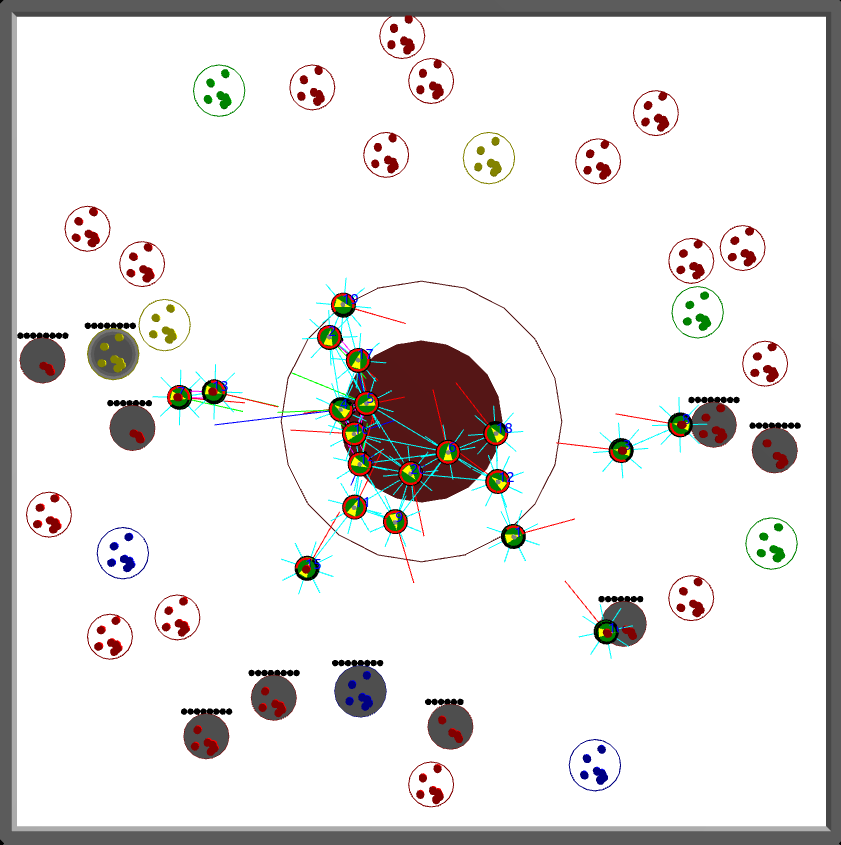
\includegraphics[width=0.66\textwidth]{top.png}
%   \caption{The ARGoS experimental environment. Resource patches are shown with the respective quality color. Patches shown with a gray background have been scouted and are included in the blockchain. The quantity of resources in blockchain-included patches is represented the black dots above them.}
%   \label{fig:arena}
% \end{figure}

\begin{figure}
\centering
\begin{minipage}{.495\textwidth}
  \centering
  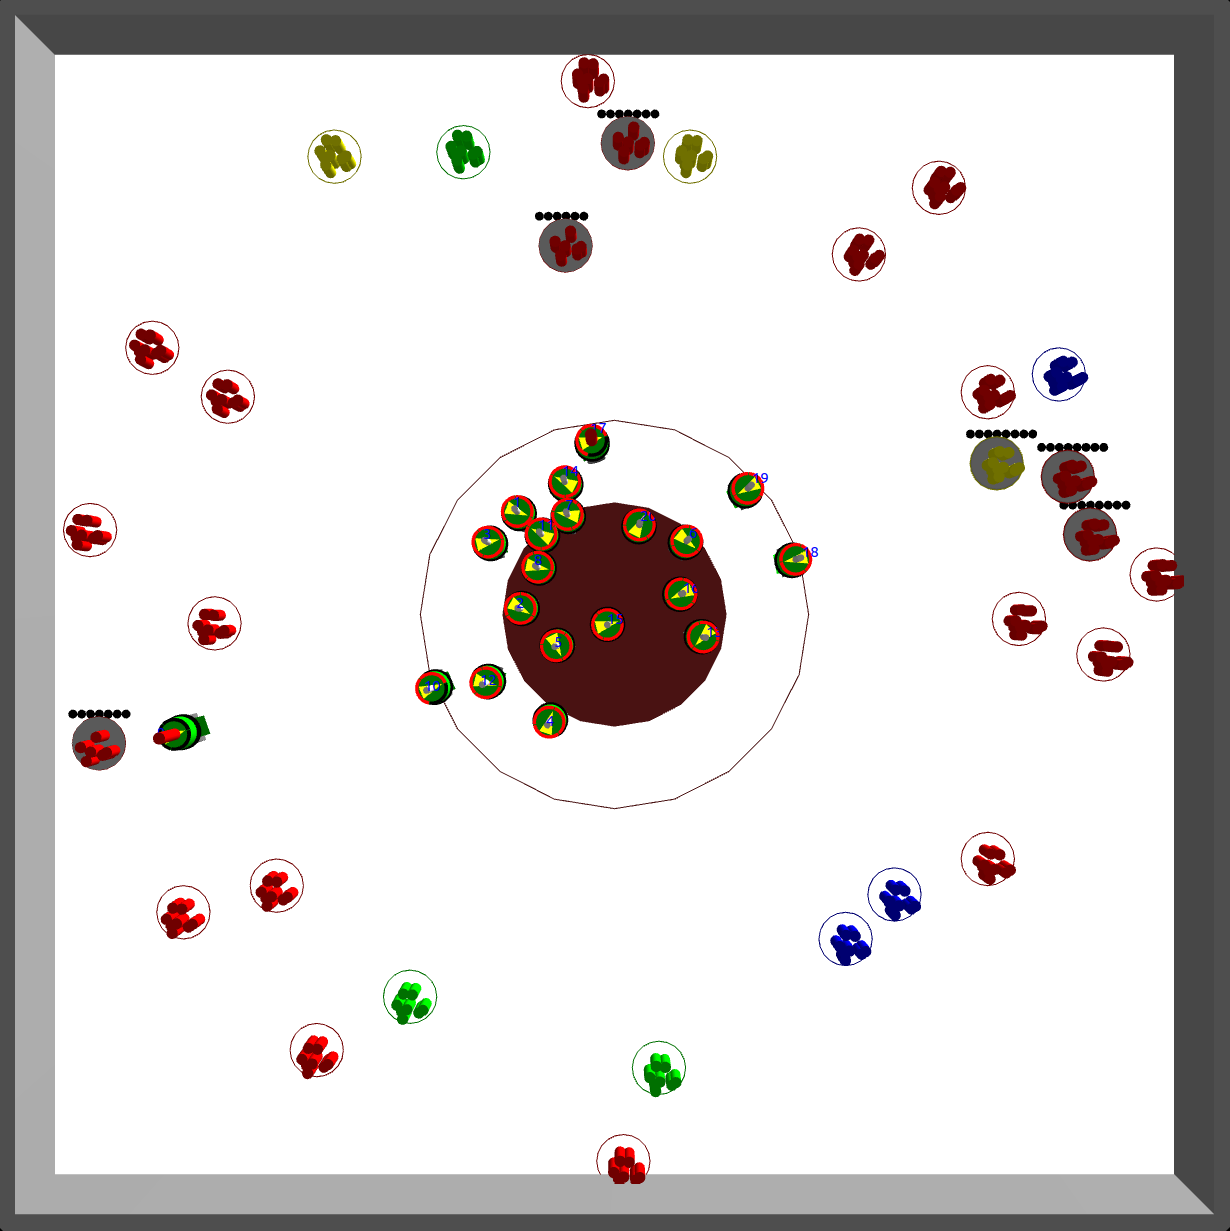
\includegraphics[width=\textwidth]{abundant.png}
  \caption{Abundant distribution}
  \label{fig:abundant}
\end{minipage}
\begin{minipage}{.495\textwidth}
  \centering
  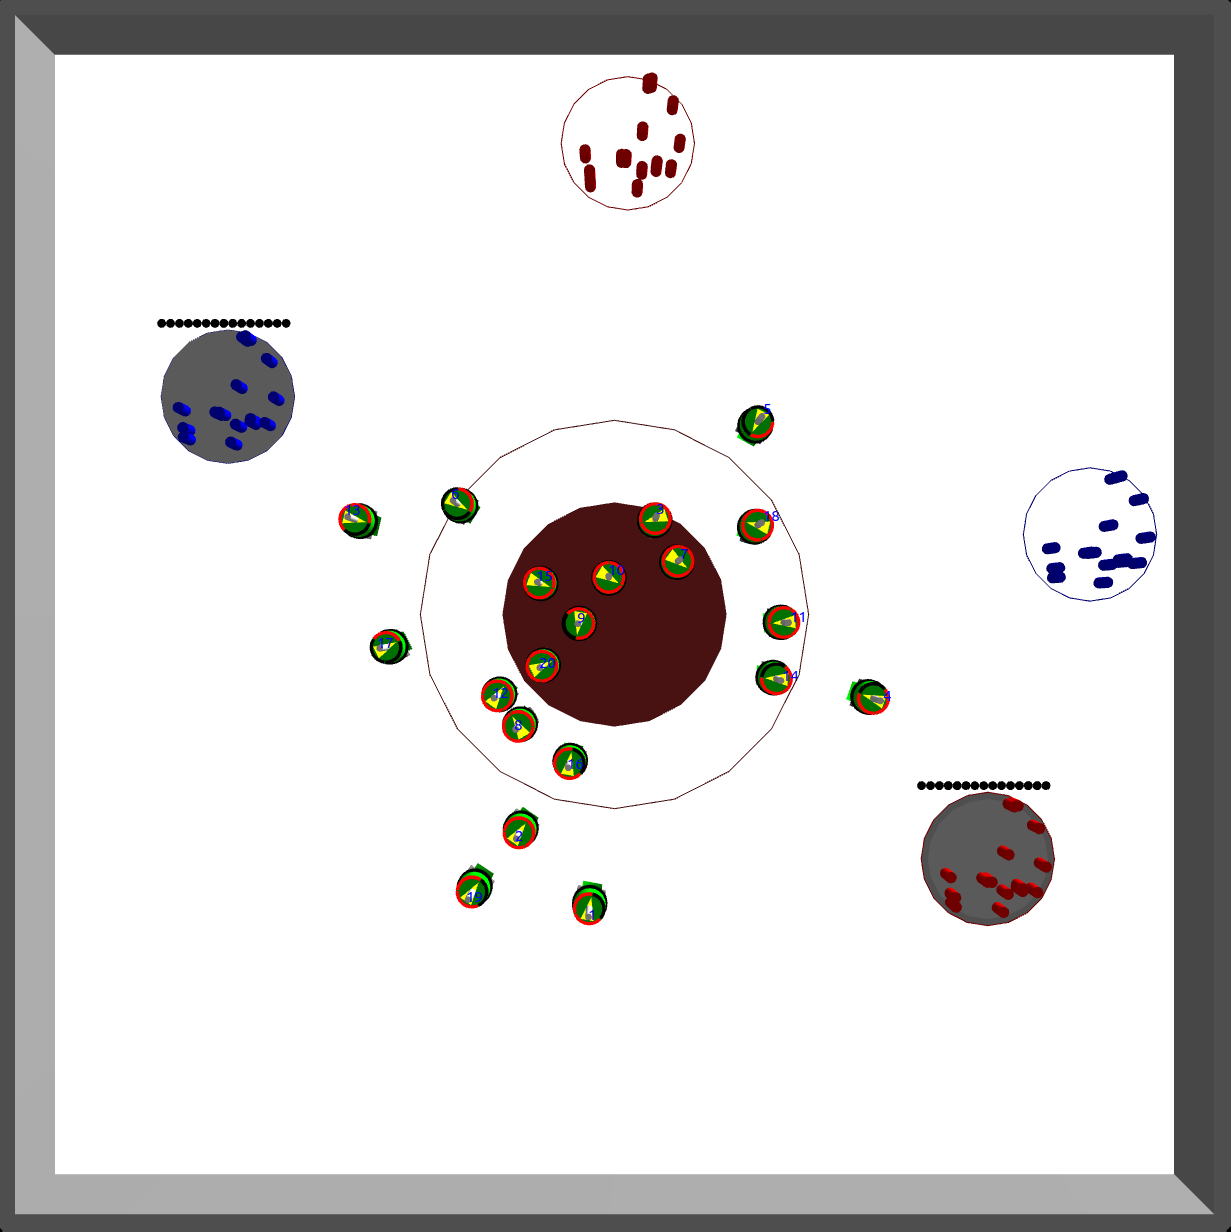
\includegraphics[width=\textwidth]{scarce.png}
  \caption{Scarce distribution}
  \label{fig:scarce}
\end{minipage}
\end{figure}

\begin{figure}
\centering
\begin{minipage}{.495\textwidth}
  \centering
  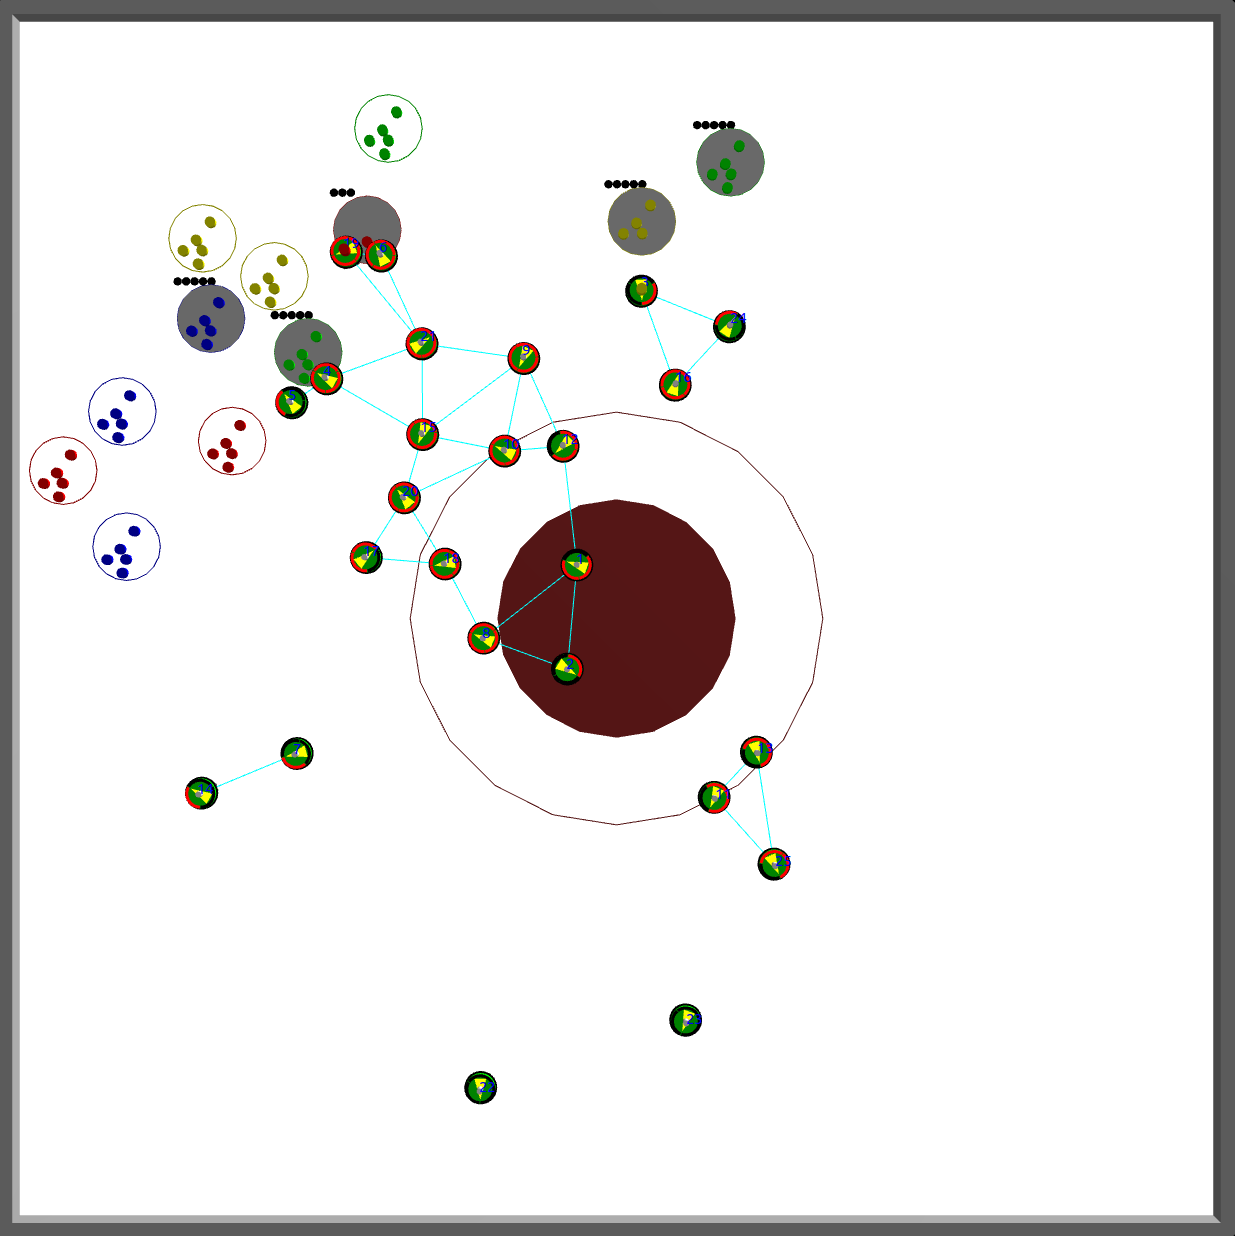
\includegraphics[width=\textwidth]{hotspot.png}
  \caption{Hotspot distribution}
  \label{fig:hotspot}
\end{minipage}
\begin{minipage}{.495\textwidth}
  \centering
  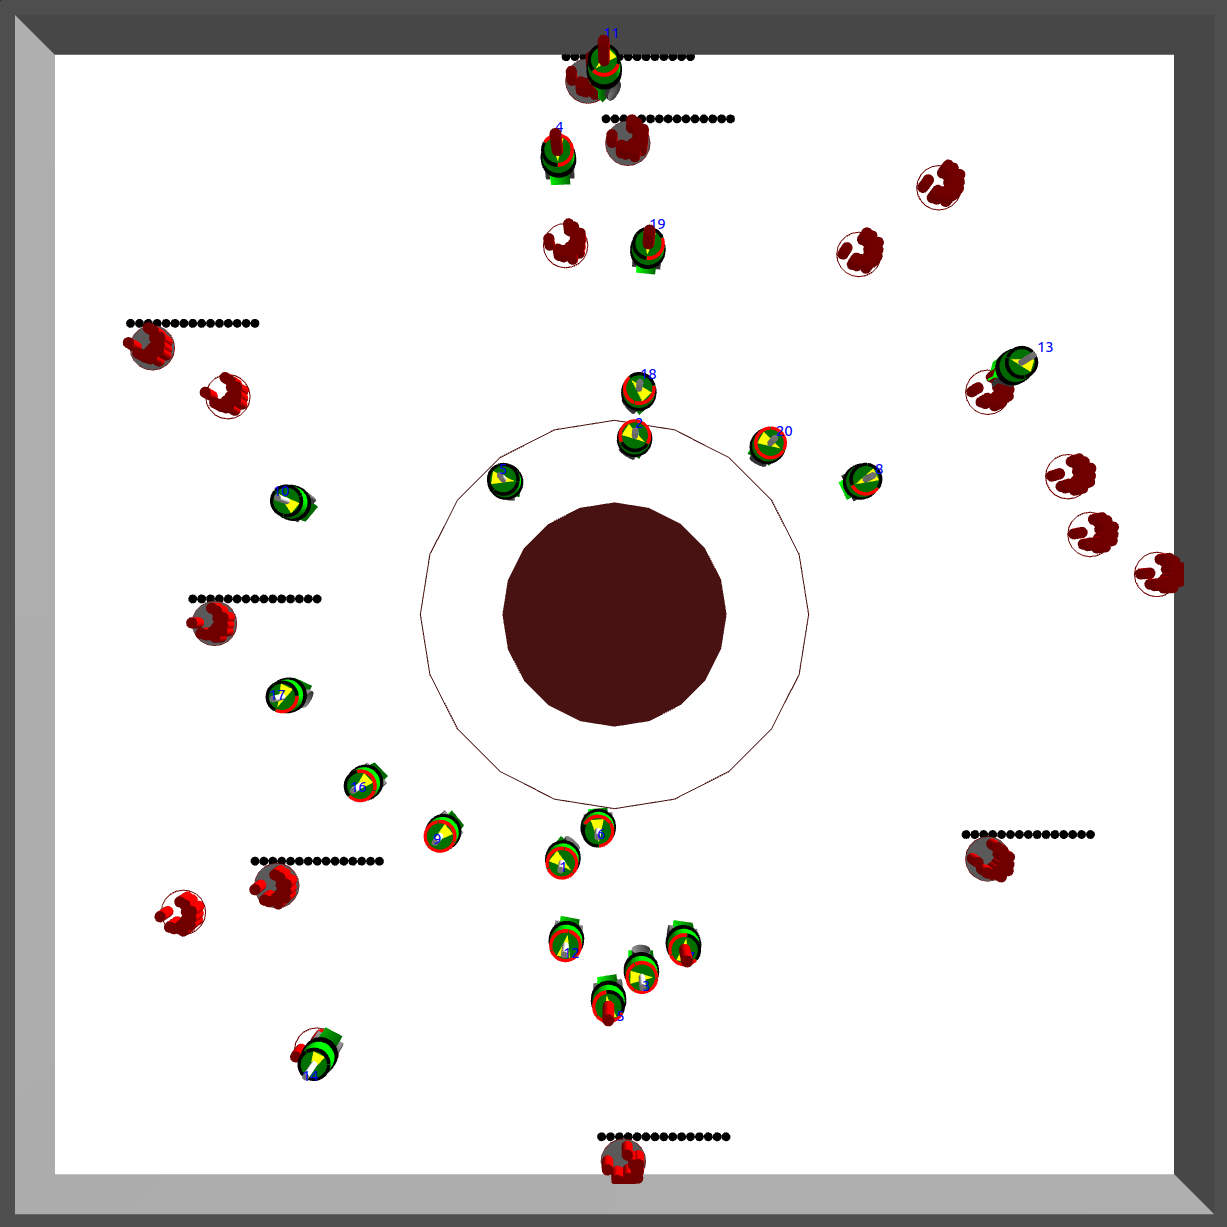
\includegraphics[width=\textwidth]{litter.png}
  \caption{Litter distribution}
  \label{fig:litter}
\end{minipage}
\end{figure}

\subsection{Description of the simulations setup}

The simulation setup comprises the swarm robotics simulation software ARGoS [arg]; and blockchain software Ethereum [vit]. Docker [doc] is used to create virtual containers which execute the nodes of a custom Ethereum network and host via TCP the Ethereum client interface called \texttt{geth} [ref]. Each ARGoS robot controller is associated with a Ethereum node and can interact with the Ethereum client using the TCP server.
Using this setup, the simulator runs smoothly since the ARGoS controllers interact with the Ethereum client to send transactions and make queries, while the execution of the Ethereum core, which maintains and synchronizes the blockchain, is performed by the docker containers in the background.
 
 To unify these components into a tool, we use Python wrappers for both ARGoS [ref], and \texttt{geth} [ref]. In this way, the Python blockchain client \texttt{web3} can be imported by the ARGoS controller and its methods (such as \texttt{add\_peer}, \texttt{send\_transaction}, etc) can be called by robot controllers written in Python. Data analysis and plotting is also performed using Python. A full description of the simulations setup can be found in [ref], and can be downloaded from [link].

\subsection{Description of the blockchain}
 Ethereum \cite{ethereum_online}, launched in 2015, extended the original application of blockchains from decentralized financial ledgers to decentralized computing platforms. While financial ledger blockchains, such as Bitcoin [nak], allow participants to agree on the execution of financial transactions, participants in the Ethereum network can also agree on the execution of computers programs known as \emph{smart contracts}. Due to their decentralized nature, blockchains require a \emph{consensus protocol} in order to solve conflicts and agree on the same version of the blockchain.

It is precisely these abilities to decentrally agree on 1)~which information is added to a common database; and 2)~on the orderly execution of smart contracts, which we argue can be very valuable for the coordination of robot swarms.

\subsubsection{Consensus Protocol}
\label{sec:consensus-protocol}
\Pow~\cite{bitcoin_online}---the original and most commonly used blockchain consensus protocol---requires the expenditure of computational resources to establish which blocks of information are added to the blockchain. For this reason, it is often regarded as counter-indicated for swarm robotics applications, which are typically energy limited [ref].
In our research, we introduced \poa [poa] as an alternative to \pow. \Poa keeps a core of authorized and accountable nodes which share the role of producing (sealing) new blocks. In this protocol, anyone can create a block and propose it, but in o``rder for a new block to be valid:
\begin{itemize}
\item the difference between the timestamp of the new block must be at least $t=B_p$ seconds ($t=B_p$ is called the \emph{block period});
\item a sealer can only sign one block every $\floor{\frac{N}{2}} + 1$ blocks
  (to guarantee majority voting in a network with $N$ sealers);
\item a sealer must create a correct signature using its private key and sign the hash of the current block.
\end{itemize}
The nodes in the network check these conditions for every block. If the conditions are met, the node appends that block to its local copy of the blockchain. The consensus protocol establishes that the current version of the blockchain is the one which has the highest \emph{cumulative difficulty}. Blocks which are sealed \emph{in-turn} (i.e., that are sealed by an appointed preferred sealer for that block), contribute with a difficulty of 2; while other blocks contribute with 1.

Blockchain forks can occur temporarily, for instance, when preferred sealers are unavailable in a partitioned network or when there is excessive communication delay. To increase the confidence that information is permanently added to the blockchain, nodes can wait for the cumulative difficulty to increase. Unreliable sealers (faulty robots for instance) can be voted out by majority vote, and new sealers may also be voted in. As such \poa is suitable for dynamic swarms, in which robots can join and leave the swarm during the execution of the collective task.

\subsubsection{Blockchain-Based Smart Contract}
\label{sec:smart-contract}

A blockchain-based smart contract is a computer program that is stored on the blockchain. It encapsulates code (its functions) and data (its state), and participants of the blockchain network are able to alter its state by sending transactions to its functions. 

The smart contract used in this experiment allows robots:~1) to store information regarding discovered resource patches (patch location with reference to the nest, as well as the quantity and quality of resources);~2) to enlist themselves as recruits to resource patches; and~3) to query information about resource sites. The smart contract supervisor additionally regulates swarm behavior by establishing a limit on the number of recruits allowed per patch and combining information provided by different robots into a single database, thus reducing physical and informational interference.

Our smart contract offers three functions that the robots can interact with:
\begin{itemize}
	\item[$\bullet$] \texttt{scout(string resource\_json)} - the scout transacts a formatted string containing patch position, radius, quality and quantity of the resource. If the position is unique (within an error margin) a new resource is added to a list, otherwise the information about a current resource is updated
	\item[$\bullet$] \texttt{recruit()} - assigns the highest quality available resource to the caller (the caller becomes a recruit);
	\item[$\bullet$] \texttt{get\_resources() return list} - returns a list with all resources and relevant information about them (including the scout and current recruits).
\end{itemize}

\subsection{Description of the robot model (Pi-puck)}
The agent used in the simulations is a model of the Pi-puck robot [york]. In previous research, we showed that 1)~the pi-puck robots are capable of executing the blockchain software [me]; and 2)~that the simulation setup we use provides an accurate approximation of the real swarm behavior [volk]. 

% Probably can save a few lines here, too much information about the robots
The simulated pi-puck integrates models of the actuators and sensors which the robots require for this experiment: infrared sensors which are used for obstacle avoidance; a \rab board which is used to discover peers and communicate blockchain identities; a ground sensor which detects colored resource sites when the robots move over them; and two motors which are used for motion. The real robot has no gripper or actuator to manipulate foraged resources, as such resource collection and depositing is performed virtually. % or abstracted?
 
\subsection{Description of the robot controller}
The robots are controlled through a \emph{finite-state-machine} composed of 6 states. At each simulation step, the robot performs a routine according to its current state and verifies the transition conditions. Additionally, the \emph{blockchain peer discovery} is performed at the beginning of every simulation step, regardless of the robot state.

\subsubsection{Finite state machine}
\label{sec:finite-state-machine}
\begin{itemize}
\item \texttt{Idle.IDLE} - The robot waits for a fixed amount of time ($30$~seconds) and then transitions to \texttt{Scout.EXPLORE};
\item \texttt{Idle.PLAN} - The robot queries \texttt{get\_resources() return list}. If the robot is enlisted as a recruit, it transitions to \texttt{Recruit.FORAGE}. Otherwise, the robot transitions to \texttt{Recruit.TRANSACT};
\item \texttt{Scout.EXPLORE} - The robot performs a random-walk for an amount of time taken from an normal distribution $\mathcal{N}(\mu=26,\sigma=5)$ and records the scouted resources locally. Afterwards, it transitions to \texttt{Scout.TRANSACT};
\item \texttt{Scout.TRANSACT} - The robot transacts \texttt{scout(string resource\_json)} for each scouted resource and deletes it from local storage. After the last transaction is successfully included in a block and confirmed (minimum 3 blocks), it transitions to \texttt{Idle.PLAN};
\item \texttt{Recruit.TRANSACT} - The robot transacts \texttt{recruit()} to be assigned a new resource for foraging. If the transaction is successfully included in a block and confirmed (minimum 3 blocks), it transitions to \texttt{Idle.PLAN}. Otherwise, there are not resources available and the robot transitions to \texttt{Idle.IDLE};
\item \texttt{Recruit.FORAGE} - The robot navigates from the nest towards the direction of the resource and searches the neighbourhood for $10$~seconds or until a resource is found a collected. Afterwards, the robot returns to the nest and transitions to \texttt{Scout.TRANSACT}.
\end{itemize}

\subsubsection{Blockchain peer discovery}
\label{sec:peer-discovery}
Our blockchain peering scheme serves two purposes: 1)~to ensure that communications are only local and thus mimic a real-world swarm deployment where network partitioning can occur; and 2)~to provide an additional layer of security which prevents external agents from participating in consensus as the robots reject connections which are not accompanied by the short range greeting.
The robots use the \rab board to broadcast their IP address (up to $30$~cm). If this communication is reciprocated, each robot send its enode via TCP. The enode is an unique identifier that the robots use to add and remove peers using \texttt{geth}. After the short range signal is lost, each robot deletes the peer from local memory and removes them using \texttt{geth}. 

\section{Results and Discussion}
\label{sec:results-and-discussion}

The main advantage of deploying a blockchain lies in the ability to optimize the swarm behavior by aggregating important information from the robots and leveraging this information to coordinate the robots' actions, while maintaining important properties of a robot swarm, such as \emph{decentralization}, \emph{adaptability} and \emph{scalability}.

The blockchain allows robots to agree on the state of the environment and on a shared coordination strategy, without the need for delegated supervisors (in contrast with centralized or hybrid control). Instead, the blockchain enables a decentralized and democratic swarm, in which all robots contribute homogeneously to the decision-making process. Such a system is robust to network partitioning, and can thus adapt to situations where a system that relies on information traveling to and from supervisors would fail (for example, in environments with limited or no communication infrastructure). 

The catch lies in the form of \emph{consensus latency}, i.e., the time it takes for messages to travel between robots and to be verified in this democratic process---and in \emph{data storage costs}, since each robot keeps a local copy of the blockchain database. These aspects raise scalability concerns in terms of communications and hardware requirements. In section~\ref{subsec:scalability} we discuss these concerns.

Cooperation is not always an advantage [pit]. Sharing information can lead the swarm to over-exploit already known resources and miss out by not exploring for better resources. It also leads to higher physical interference (due to increase robot collisions) and informational interference (due to the broadcasting of incorrect/outdated information). The role of a supervisor is to optimize the foraging task (in terms of total reward collected and/or energy efficiency) by aggregating the latest known information from robot scouts and allocating resources to robot recruits, thus minimizing the impact of interference. In section~\ref{subsec:performance} we show the performance results of a blockchain-coordinated robot swarm in comparison with an uncoordinated swarm, in environments with different resource distributions, and as the maximum number of recruits allowed by the smart contract increases.

%In results section A, we compare two robot swarms in which the individual robots perform the same control routine, but with one key difference: one swarm does not use a blockchain and thus the robots forage resources based on their own scouting and local data. In contrast, the robots in the second swarm do not keep any information locally. Instead, they transact to store the resource information on the blockchain and perform foraging based on the information that they have added to the blockchain. In this fashion, we seek to draw conclusions regarding the aforementioned scalability concerns of a blockchain-controlled approach to swarm coordination.

%In experiment B, we analyze the performance of a $20$~robot swarm performing the foraging task using blockchain supervisory control in the different resource distributions described in~\ref{subsec:env}. We expect that in some distributions the swarm will benefit more from the integration of blockchain supervision than in others.

\subsection{Scalability}
\label{subsec:scalability}

\subsubsection{Consensus latency}

 Figure~\ref{fig:block-histograms} (top) shows the \emph{Block Reception Time}, which is the difference between the timestamp at the moment a robot receives a block, and the timestamp at the moment it is produced (in other words, the time it took for a block to be disseminated from its producer to every other node). Figure~\ref{fig:block-histograms} (bottom) shows the \emph{Block Production Time}, that is the difference of the timestamps between two consecutive blocks on the final version of the blockchain. Both these metrics are obtained offline and post-experiment.
 
The \emph{block period} parameter sets the minimum required difference between the timestamps of two consecutive blocks (see \ref{sec:methods}), and thus has a big effect on the information delay introduced by the blockchain: if it is too high, it reduces the possibility to employ the shared knowledge to perform time-critical tasks. Conversely, if it is too low, it increases the frequency of block production which leads to~1) higher costs of communication, computation and data storage; and~2) increased rate of blockchain forks which contain redundant, or more dangerously, conflicting information.
 
 In figure~\ref{fig:block-histograms} (top) we observe that an majority of blocks are received within $2$~seconds. This observation justifies our choice of a block period $T_{block}=2s$, as there is a high chance that the previous block has been disseminated through the network before it is time to produce the next block (thus reducing the number of forks).

\begin{figure}
  \centering
  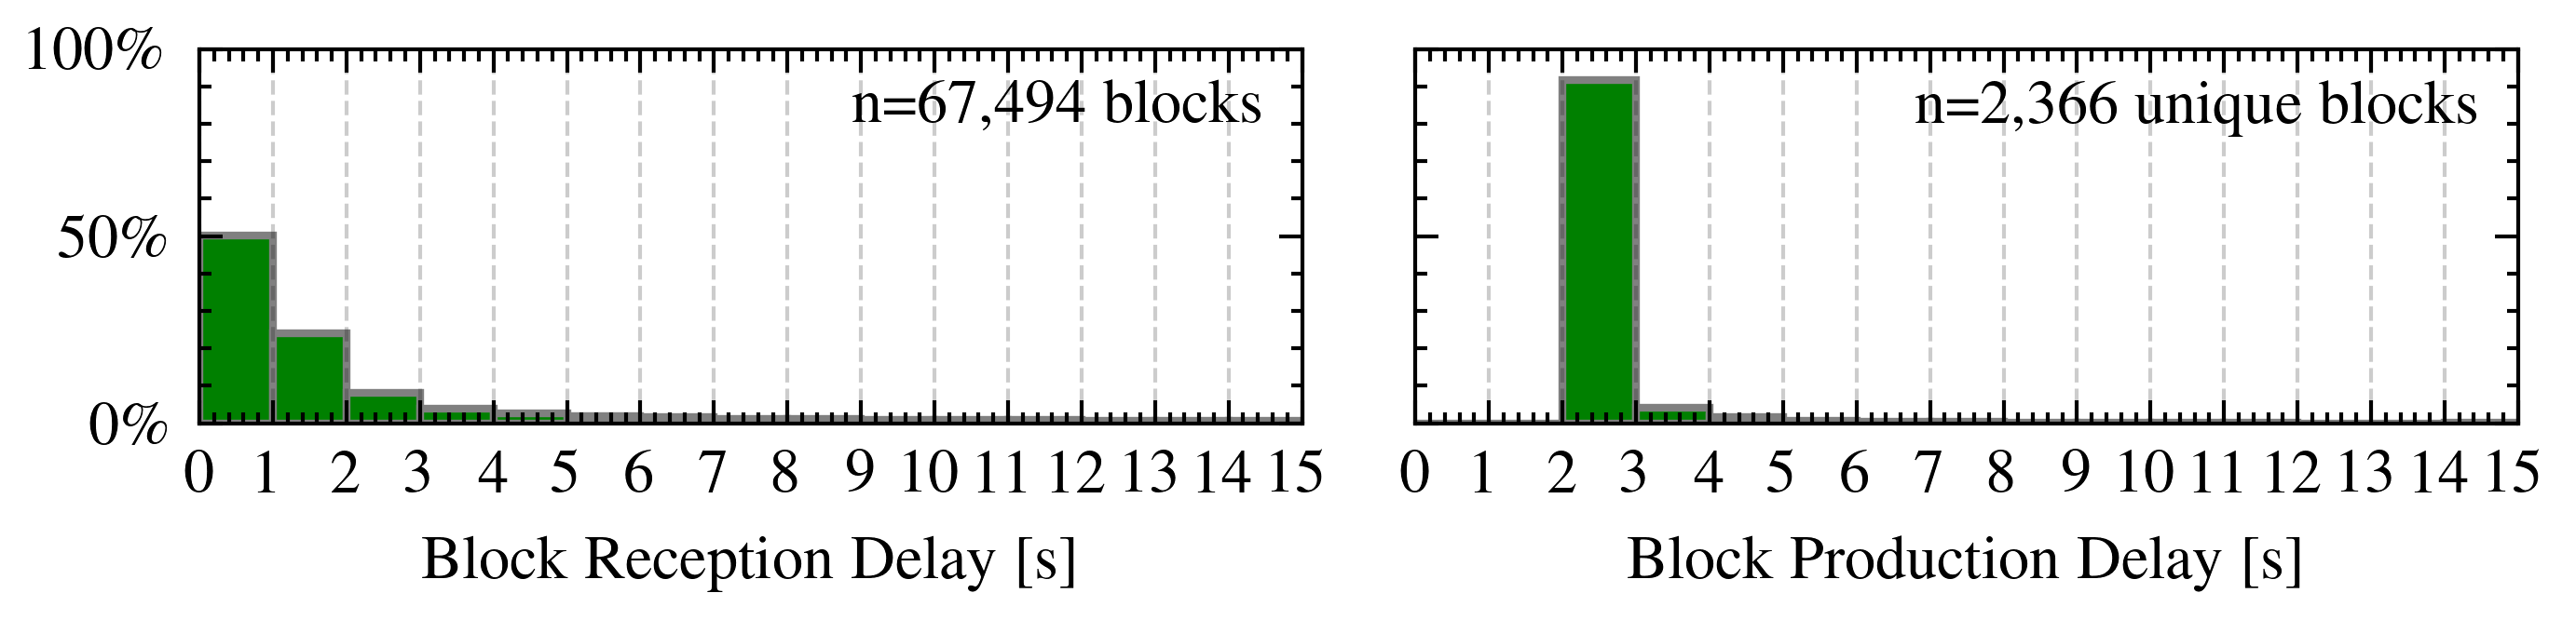
\includegraphics{multi/time_elapsed_both.png}
  \caption{Top: The time it took for every robot to receive each new block of information. In our experiments, 60\% of the blocks were consistently received in under $2$~seconds, which justifies the choice for a block period $T_{block}=2s$. Bottom: The time it took for a new block to be produced. With $T_{block}=2s$, the minimum and ideal production delay is $2$~seconds. An additional delay is introduced due to network delays (temporary unavailability of the preferred block producer, for instance). In our experiments, 90\% of the blocks were produced within $2$~-$3$~seconds, which means that the blockchain is working under nominal conditions throughout all experiments. Note: these plots are generated from the combined data of all experiments performed in this study}
  \label{fig:block-histograms}
\end{figure}

\subsubsection{Data storage cost}

In previous research [me,volk], the block period was $15$~seconds. With a block period of $2$~seconds, we expect that the costs of storing the blockchain will be higher since the amount of data stored depends on the number of blocks created, and also on number of transactions executed by the robots. 

Figure~\ref{fig:data-storage} shows the size (in MB) of the folder where the blockchain is stored. The data storage increases linearly over the course of the experiment, and sublinearly with the number of robots in the swarm. At the end of the experiment, the occupied card storage is about $8$~MB (for reference, our experiment carried out on a $16$~GB SD could be performed $2000$~times before running out of storage space). Furthermore, in a real deployment, the robots would not need to store locally the entire history of the blockchain, as it contains outdated information which is no longer relevant for their operation. The role of storing the blockchain's history can be distributed between robots, or externally uploaded as connectivity becomes available, while the robots may still leverage blockchain cryptography to verify that their current blockchain segments are consistent with the complete blockchain history.

To summarize, we do not expect memory to pose an scalability problem in a real deployment because: 1)~the cost is reasonable given current data storage technology; and 2)~blockchain technology can be leveraged to reduce the storage costs in robot swarms.

\begin{figure}
  \centering
  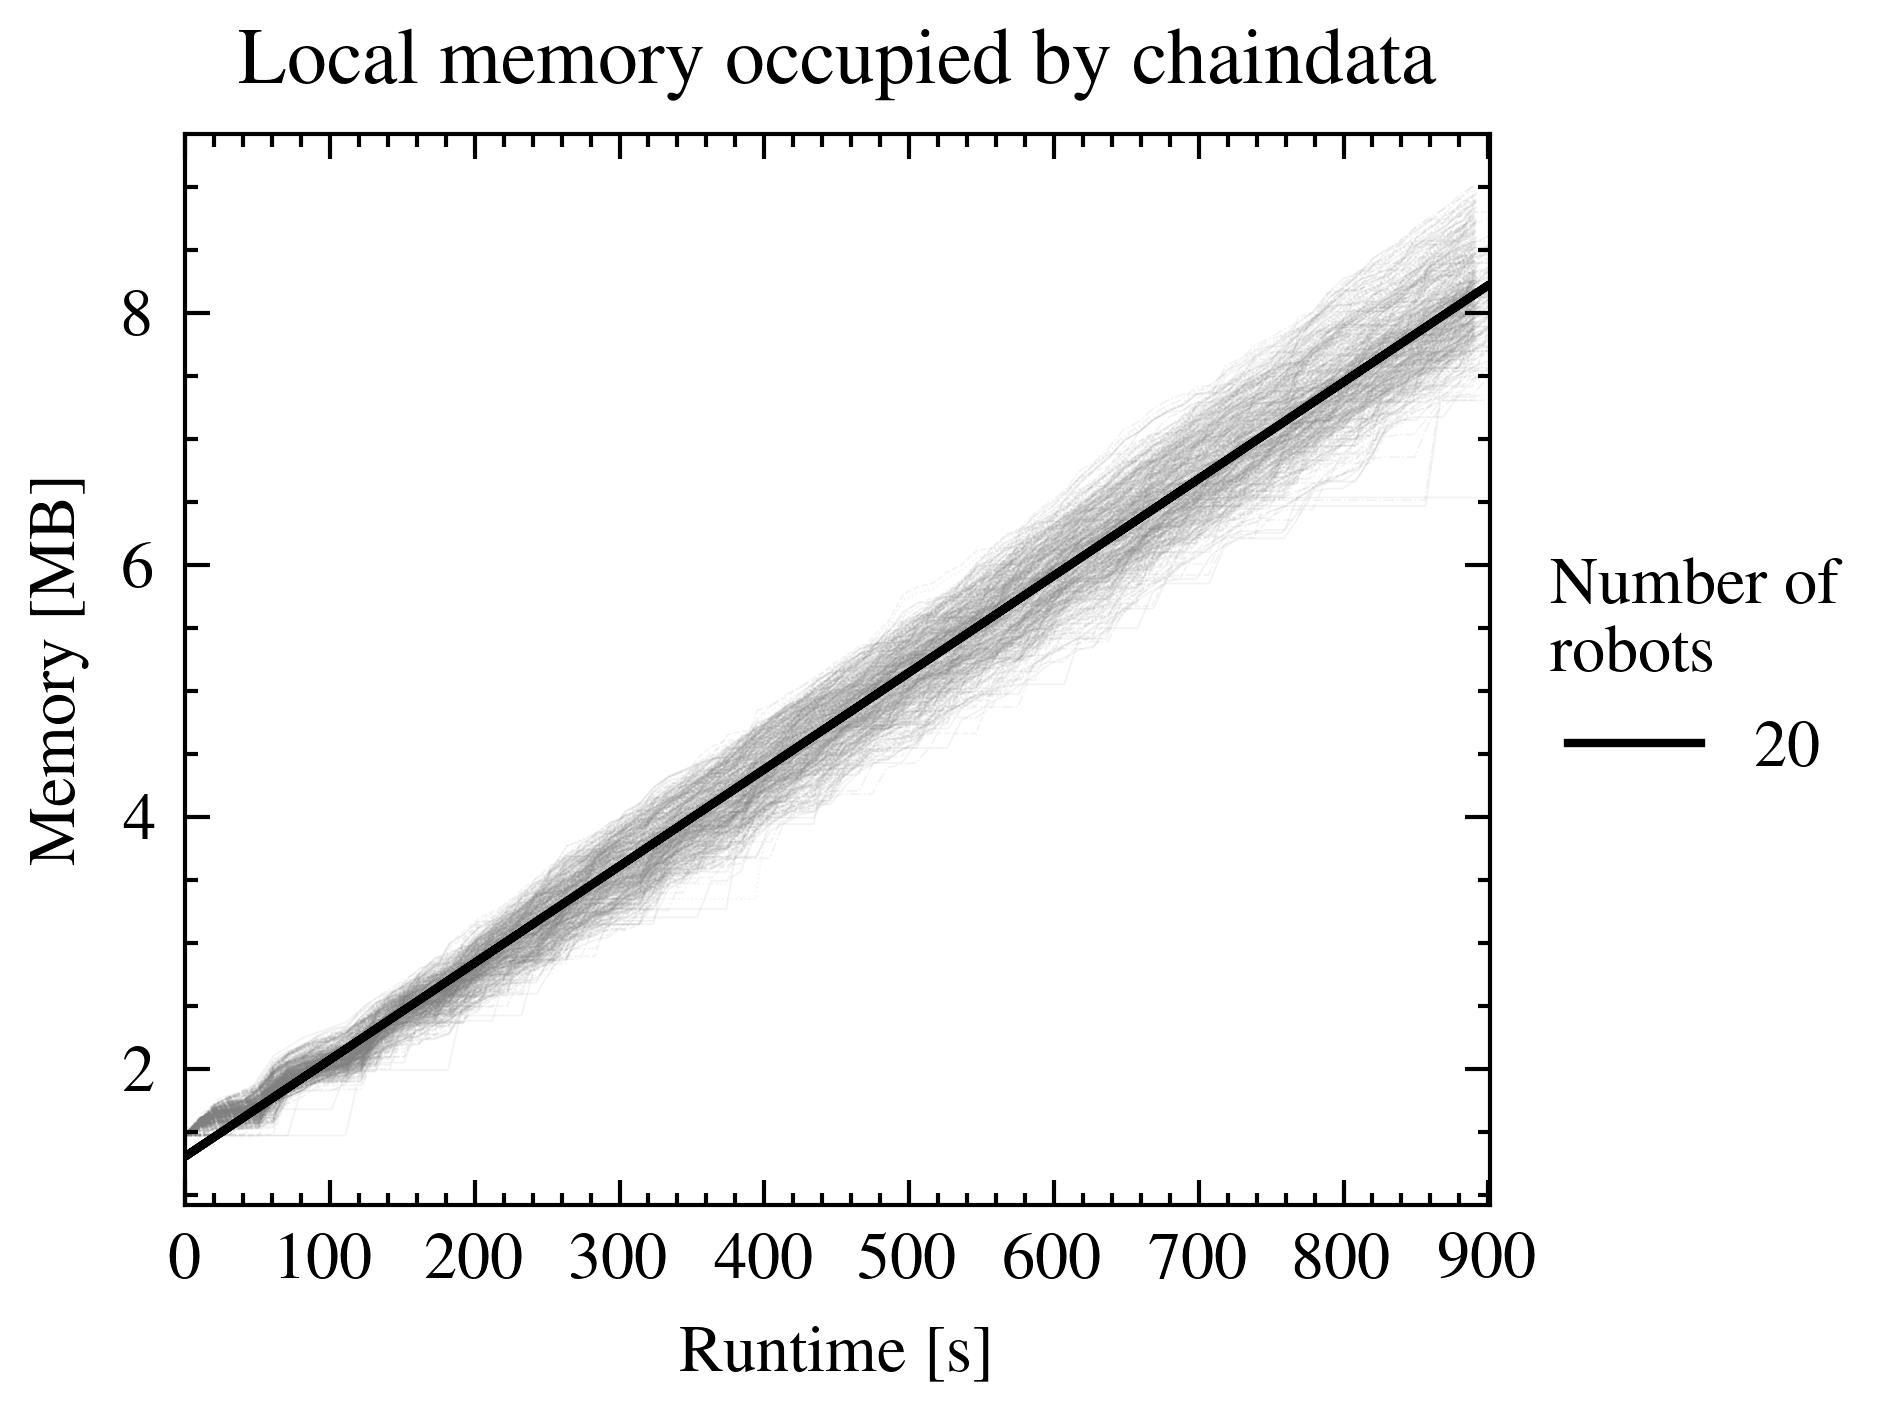
\includegraphics{test116_rich/local_memory.png}
  \caption{The storage space occupied by the blockchain grows linearly over time. The lines in gray are the exact values over time; while the colored lines are linear regressions for three different swarm sizes over $20$~repetitions \todo{change memory to Data storage costs, maybe add 25 and 30 robot experiments}} 
  \label{fig:data-storage}
\end{figure}


%To analyze the impact on performance of the delay introduced by the blockchain on the swarm, we apply the same controller -- individualist controller.
%\begin{figure}
%  \centering
%  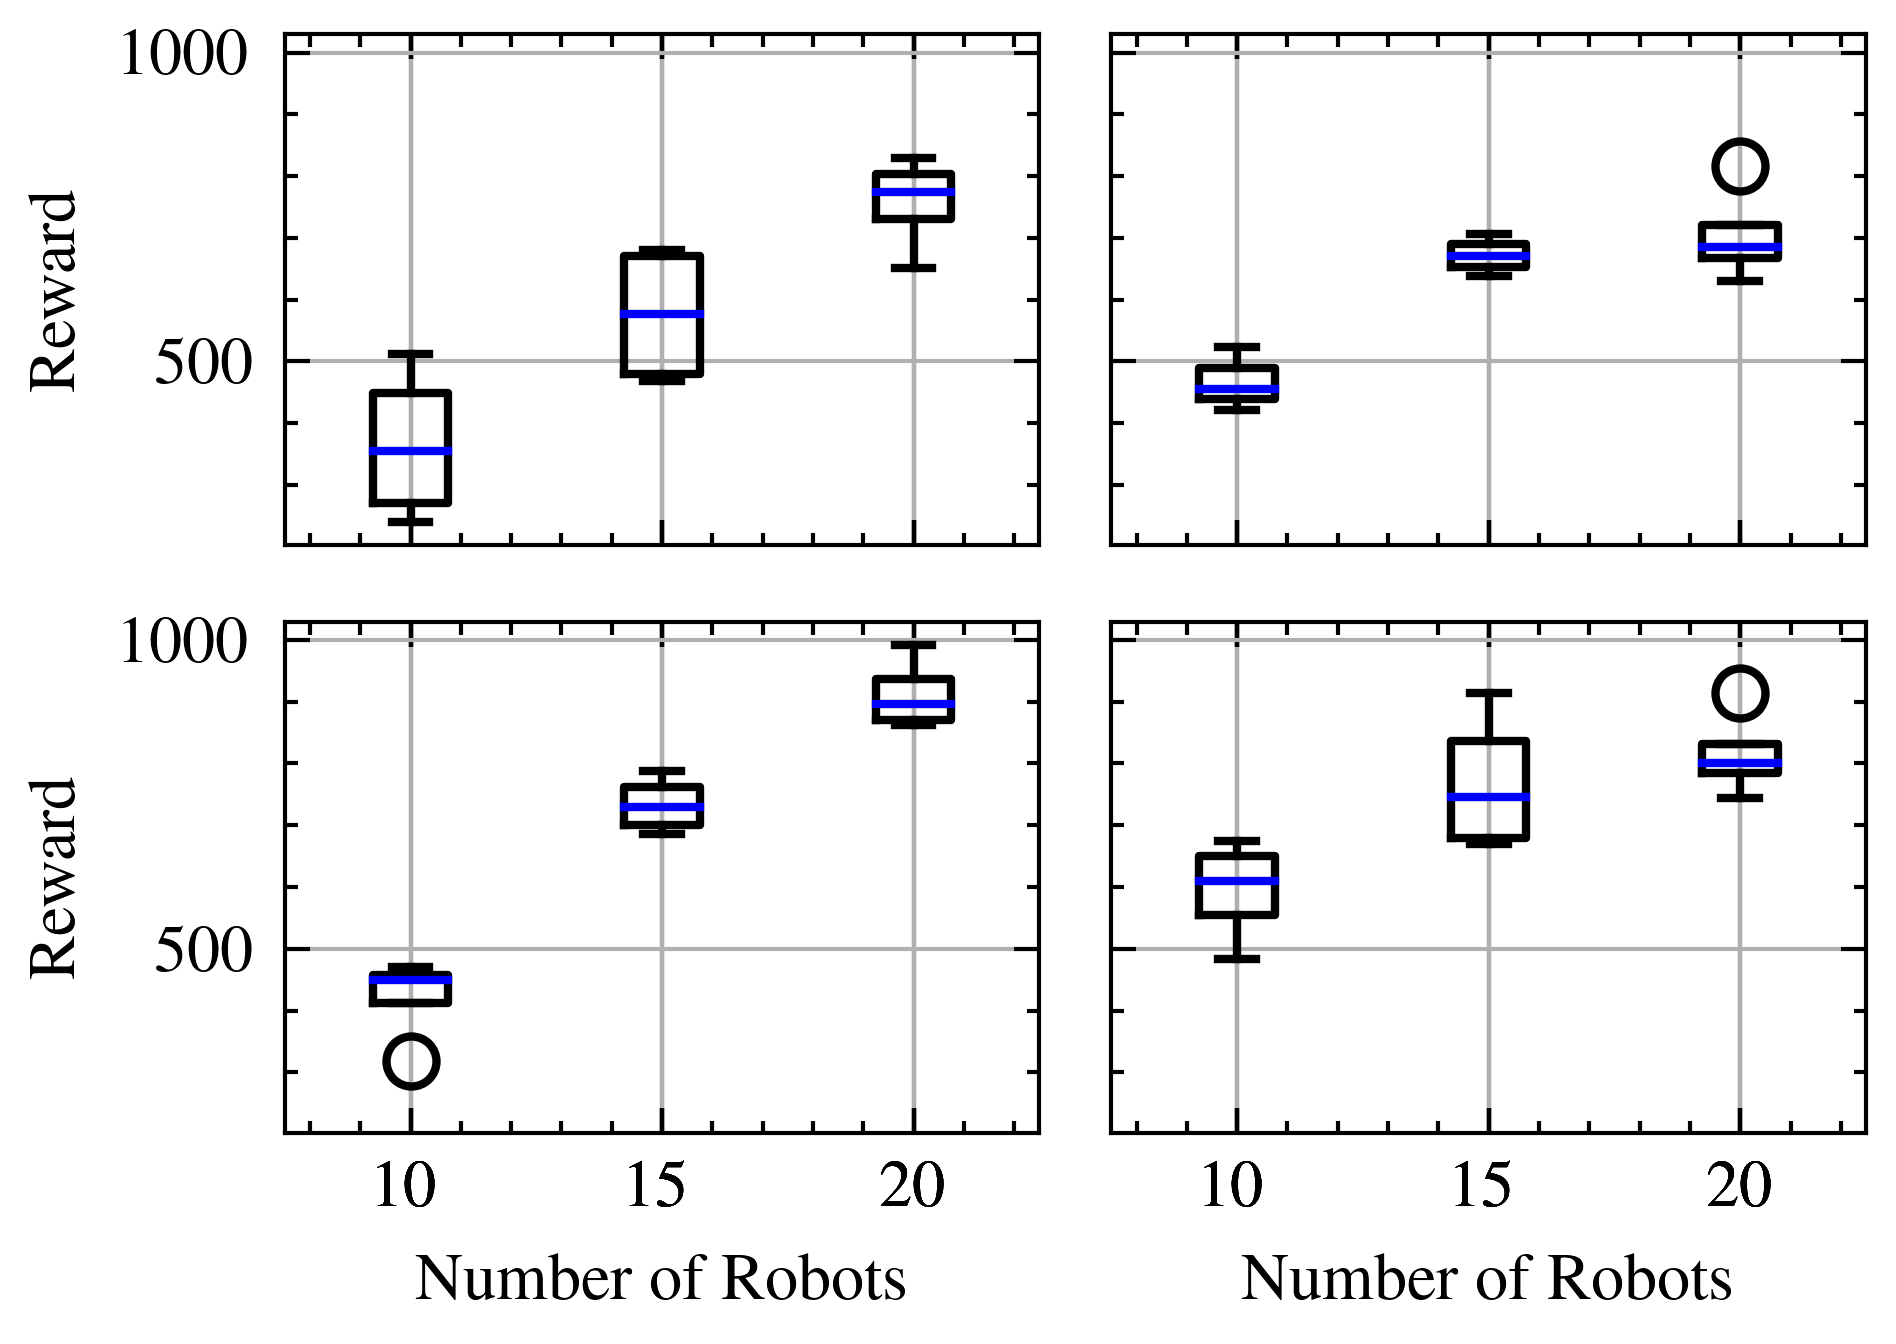
\includegraphics{test116/value_bp_Robots.png}
%  \caption{} 
%  \label{fig:experiment3}
%\end{figure}
%\begin{figure}
%  \centering
%  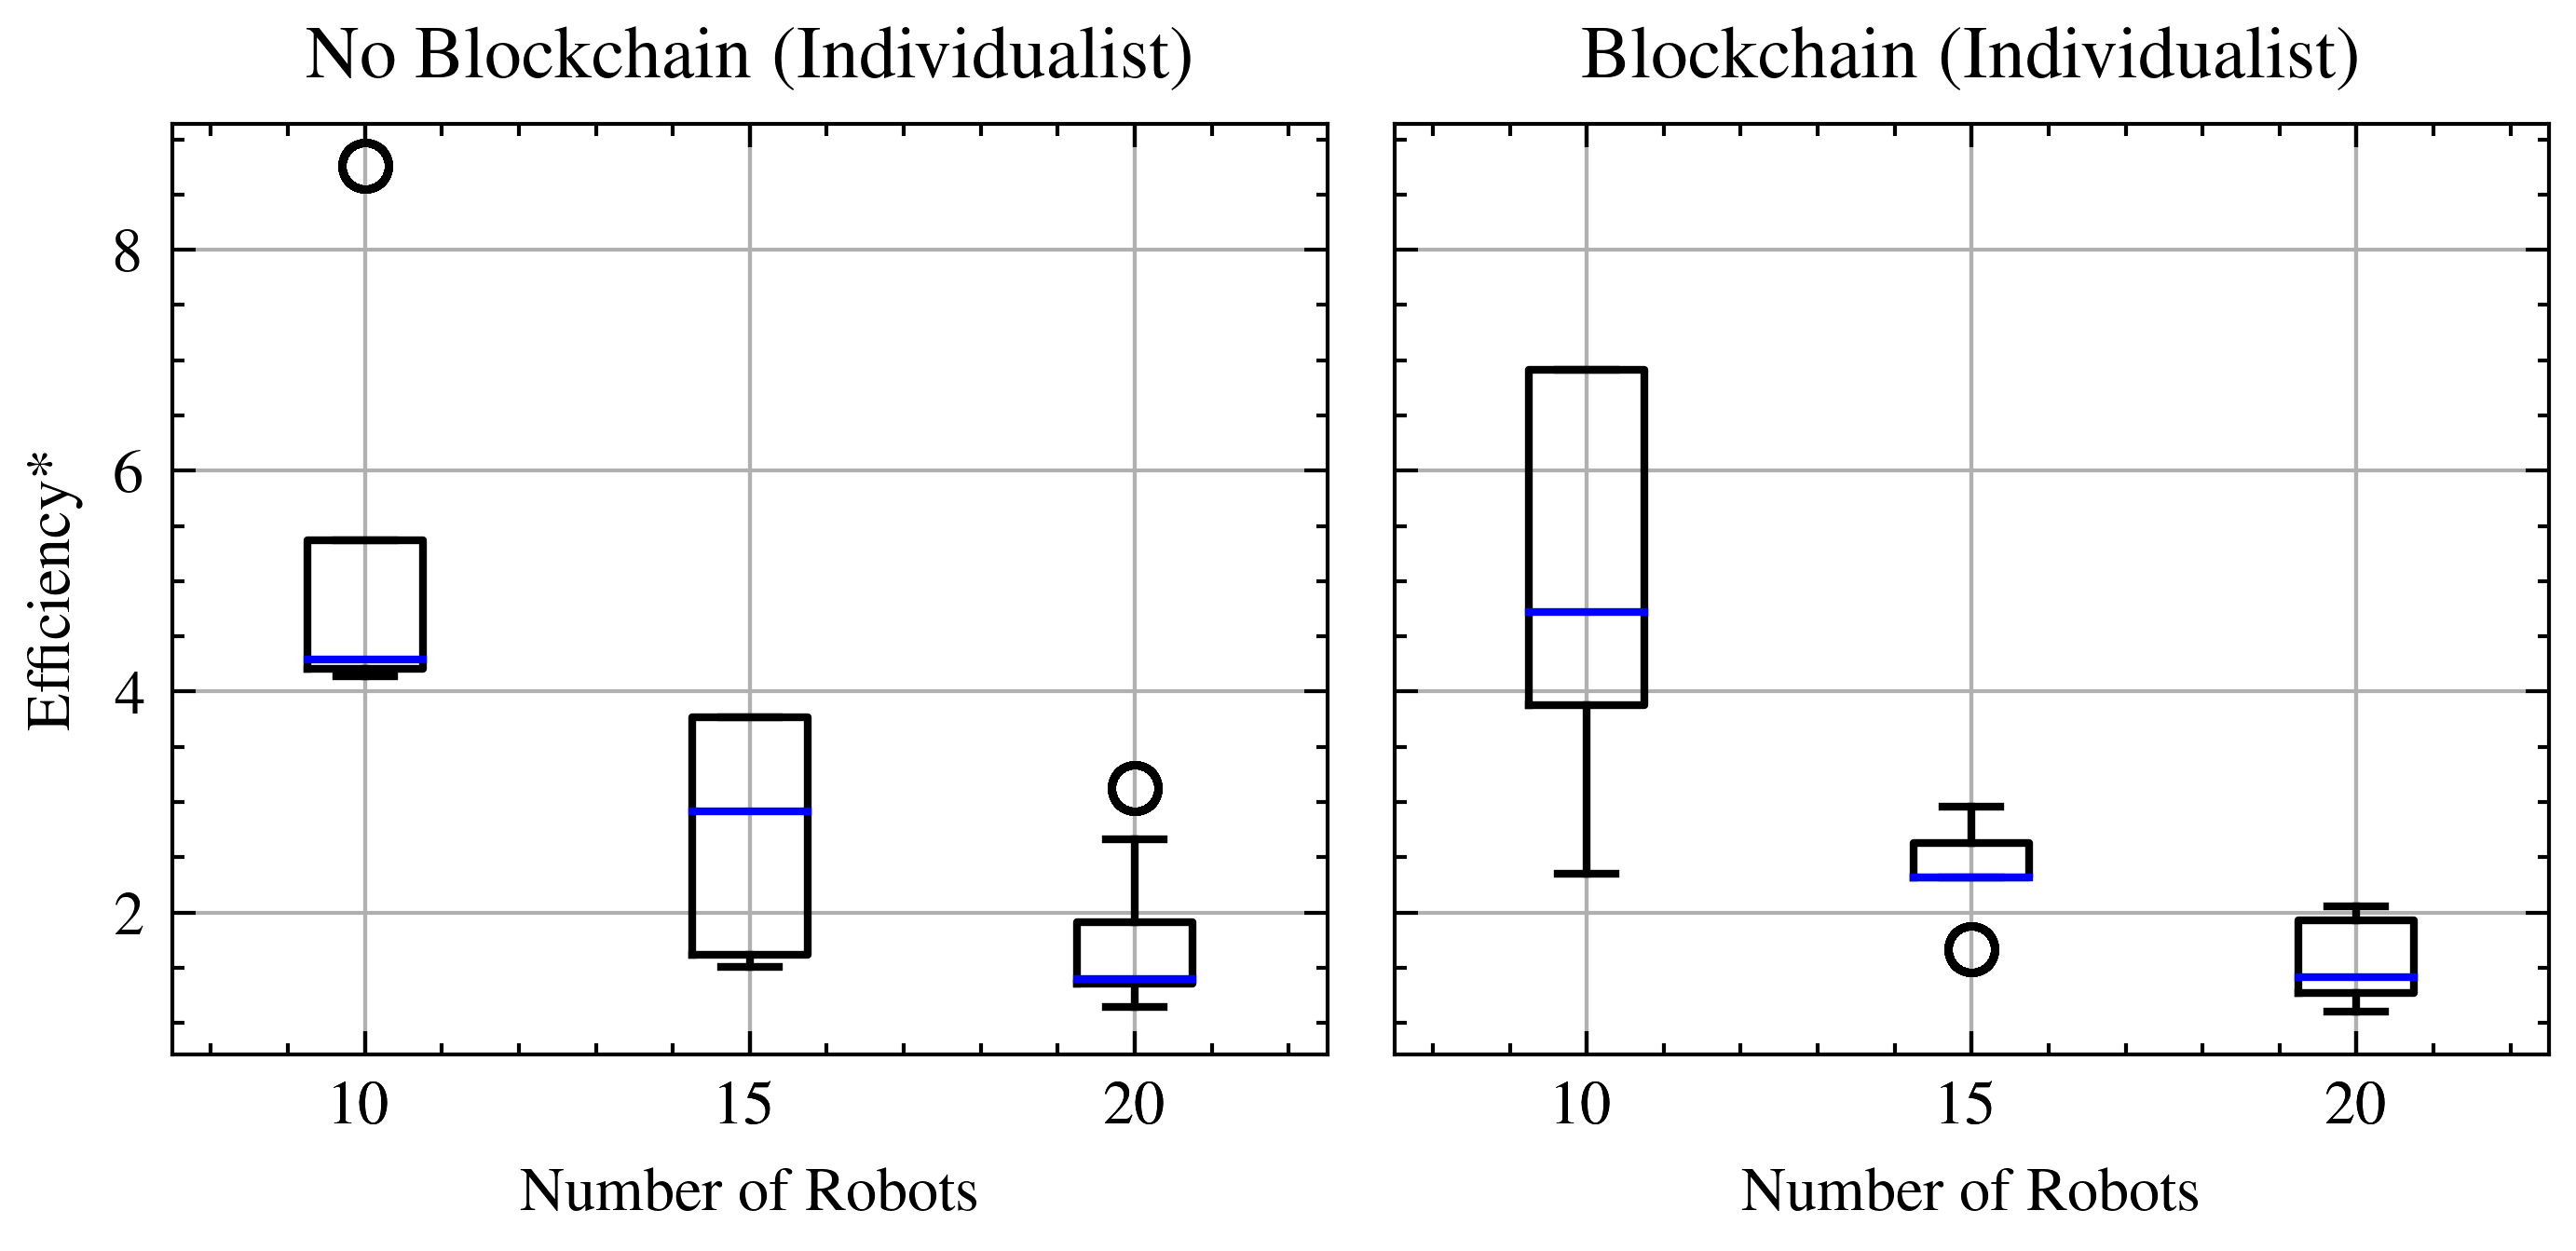
\includegraphics{test116/efficiency_bp_Robots.png}
%  \caption{} 
%  \label{fig:experiment3}
%\end{figure}

\subsection{Performance}
\label{subsec:performance}

\todo{Remove some plots; Decide which stay; Combine them into single plot with subplots; Make them smaller?; fix some y labels; change 0 recruits to greedy or N/A and explain it is blockchain free approach.}

\subsubsection{Abundant distribution}
%In the abundant distribution $5$\% of the environment floor area is covered with uniformly distributed patches. Each patch has a diameter of 12~$cm$ and contains $8$~resources. 70\% of the patches are red, while there is 10\% of each green, blue and yellow.

The environment is considered abundant since it is easy for the robots to independently discover resources. In such environments, individualist foragers can perform well enough [pit, Wilson 2000], or even better if the benefits of cooperation to not overcome the damages of interference. In Figure~\ref{fig:abundant-value} the total reward collected saturates after $2$ recruits per patch, and begins to drop at $5$ recruits. Cooperating robots share the location of higher quality patches, and are thus capable of retrieving more reward with an increased scouting efficiency (Figure~\ref{fig:abundant-eff-exp}). On the other hand, as the number of recruits becomes too high (more then $2$ recruits) interference and lack of robots available for scouting start to harm the performance of the swarm overall.

\begin{figure}
\centering
\begin{minipage}{.495\textwidth}
  \centering
  \includegraphics{test117/value_bp_Recruits_VALUE.png}
  \caption{A figure}
  \label{fig:abundant-value}
\end{minipage}
\begin{minipage}{.495\textwidth}
  \centering
  \includegraphics{test117/value_bp_Recruits_DIST.png}
  \caption{A figure}
  \label{fig:abundant-dist}
\end{minipage}
\end{figure}

\begin{figure}
\centering
\begin{minipage}{.495\textwidth}
  \centering
  \includegraphics{test117/efficiency_bp_Recruits_SCOUT_DIST.png}
  \caption{Another figure}
  \label{fig:abundant-eff-exp}
\end{minipage}
\begin{minipage}{.495\textwidth}
  \centering
  \includegraphics{test117/efficiency_bp_Recruits_RECRUIT_DIST.png}
  \caption{A figure}
  \label{fig:abundant-eff-for}
\end{minipage}
\end{figure}

\subsubsection{Hotspot distribution}
%In the hotspot distribution $3$\% of the environment floor area is covered with patches following a normal distribution (0.25*1.825, 0.15*1.825) around a center point. Each patch has a diameter of 14~$cm$ and contains $8$~red berries. 

The blockchain coordinated swarm is capable to retrieve more than double the reward (Figure~\ref{fig:hotspot-value}) and be $2$~-$5$~times more efficient during scouting (Figure~\ref{fig:hotspot-eff-exp}). This occurs because the scouting robots which move in the direction of the hotspot are very successful, while others robots do not find any resources. The ability to aggregate and share information prevents unsuccessful robots from idling or wasting energy performing redundant exploration. Conversely, given the tight aggregation of resources, the foraging efficiency quickly drops as the number of recruits increases due higher physical interference between robots (Figure~\ref{fig:hotspot-eff-for}).

\begin{figure}
\centering
\begin{minipage}{.495\textwidth}
  \centering
  \includegraphics{test117_patchy_single/value_bp_Recruits_VALUE.png}
  \caption{}
  \label{fig:hotspot-value}
\end{minipage}
\begin{minipage}{.495\textwidth}
  \centering
  \includegraphics{test117_patchy_single/value_bp_Recruits_DIST.png}
  \caption{A figure}
  \label{fig:hotspot-dist}
\end{minipage}
\end{figure}

\begin{figure}
\centering
\begin{minipage}{.495\textwidth}
  \centering
  \includegraphics{test117_patchy_single/efficiency_bp_Recruits_SCOUT_DIST.png}
  \caption{Another figure}
  \label{fig:hotspot-eff-exp}
\end{minipage}
\begin{minipage}{.495\textwidth}
  \centering
  \includegraphics{test117_patchy_single/efficiency_bp_Recruits_RECRUIT_DIST.png}
  \caption{A figure}
  \label{fig:hotspot-eff-for}
\end{minipage}
\end{figure}


\subsubsection{Scarce distribution}
%In the scarce distribution $4$\% of the environment floor area is covered with uniformly distributed patches. Each patch has a diameter of 30~$cm$ and contains $15$~red berries. 

The blockchain coordinated swarm is capable to retrieve $50$\% to $100$\% more reward (Figure~\ref{fig:scarce-value}) and be $2$~-$3$~times more efficient during scouting (Figure~\ref{fig:scarce-eff-scout}). In this environment, it is hard for the scouts to find resources due to relative scarcity, but it is easier for foragers as the patches are quite large and thus inferences do not show a big impact until $4$-$5$~recruits per patch. Coordination is very valuable in such an environment.

\begin{figure}
\centering
\begin{minipage}{.495\textwidth}
  \centering
  \includegraphics{test117_scarce_big/value_bp_Recruits_VALUE.png}
  \caption{A figure}
  \label{fig:scarce-value}
\end{minipage}
\begin{minipage}{.495\textwidth}
  \centering
  \includegraphics{test117_scarce_big/value_bp_Recruits_DIST.png}
  \caption{A figure}
  \label{fig:scarce-dist}
\end{minipage}
\end{figure}

\begin{figure}
\centering
\begin{minipage}{.495\textwidth}
  \centering
  \includegraphics{test117_scarce_big/efficiency_bp_Recruits_SCOUT_DIST.png}
  \caption{Another figure}
  \label{fig:scarce-eff-scout}
\end{minipage}
\begin{minipage}{.495\textwidth}
  \centering
  \includegraphics{test117_scarce_big/efficiency_bp_Recruits_RECRUIT_DIST.png}
  \caption{A figure}
  \label{fig:scarce-eff-recruit}
\end{minipage}
\end{figure}


\subsubsection{Litter distribution}
\todo{maybe remove litter -- or make it more similar to pitanokovas for comparison (15 per patch is too much for "litter")}
%In the litter distribution $2$\% of the environment floor area is covered with uniformly distributed patches. Each patch has a diameter of 10~$cm$ and contains $15$~red berries.
 The improvement is about $50$\% in the total reward collected, and the scouting efficiency doubles for $3$ or more recruits. Due to the small size of resources, the system very prone to damage from interference as the foraging efficiency drops significantly as the number of recruits increases (Figure~\ref{fig:scarce-eff-recruit}). Generally speaking, collaborating swarms in small, sparse and low quality patches have been shown to not fare well due to the reinforced effect of informational and physical interference [pit]. Despite this, the blockchain coordinated swarm shows an improved performance, although not as drastic as in the other environments.

\begin{figure}
\centering
\begin{minipage}{.495\textwidth}
  \centering
  \includegraphics{test117_litter/value_bp_Recruits_VALUE.png}
  \caption{A figure}
  \label{fig:litter-value}
\end{minipage}
\begin{minipage}{.495\textwidth}
  \centering
  \includegraphics{test117_litter/value_bp_Recruits_DIST.png}
  \caption{A figure}
  \label{fig:litter-dist}
\end{minipage}
\end{figure}

\begin{figure}
\centering
\begin{minipage}{.495\textwidth}
  \centering
  \includegraphics{test117_litter/efficiency_bp_Recruits_SCOUT_DIST.png}
  \caption{Another figure}
  \label{fig:litter-eff-scout}
\end{minipage}
\begin{minipage}{.495\textwidth}
  \centering
  \includegraphics{test117_litter/efficiency_bp_Recruits_RECRUIT_DIST.png}
  \caption{A figure}
  \label{fig:litter-eff-rec}
\end{minipage}
\end{figure}

\section{Conclusions and Future Work}
\label{sec:conclusion}

\red{
- How much time to spend foraging or recruiting? Using blockchain to apply optimal foraging theory in a smart contract supervisor \\ \\
- How many recruits per resource site? Introduce fuzzy rules to decide the number of recruits depending on size/distance/quantity/quality etc.\\ \\
}

\blue{\lipsum[1-2]}

\bibliographystyle{splncs04}
\bibliography{mybibliography}
\end{document}
